\section{Caída libre y lanzamiento vertical de los cuerpos:}

Un caso especial de MRUV es el movimiento de los cuerpos cuando están exclusivamente sólo bajo la influencia de la fuerza de la 
gravedad. También en este apartado se supondrá que la resistencia aerodinámica del aire es insignificante (para el caso real esto 
depende de la forma del cuerpo), es decir, se supone que el cuerpo se mueve el vacío. 

\subsection{Caída libre:}

Se trata del movimiento de un cuerpo cuando cae desde cierta altura (la distancia que recorre el cuerpo durante toda la caída) 
por encima del nivel de la superficie de la Tierra (piso) hacia abajo. Este movimiento es un MRUV con una aceleración la cual es 
la gravedad $a = g = 9.8 m/s^2$ (constante), la cual está en la misma dirección de la velocidad lo cual hace que se trate de un 
movimiento acelerado. 

\begin{figure}[ht]
 \centering
 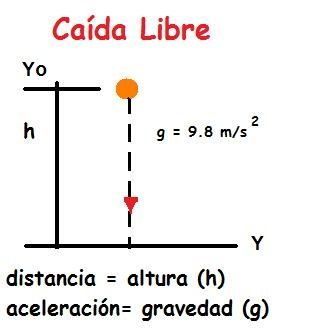
\includegraphics[scale=0.5]{images/caida-libre.jpg}
 % cinematica.png: 0x0 px, 300dpi, 0.00x0.00 cm, bb=
 \caption{Ilustración de la caída libre de un cuerpo.}\label{caidalibre}
\end{figure} 

Y las ecuaciones de movimiento son las de un MRUV:

\begin{equation}
 v_f = v_0 + gt
\end{equation}

\begin{equation}
 v_f^2 = v_0^2 + 2gh
\end{equation}

\begin{equation}
 h = (\frac{v_f + v_0}{2})t
\end{equation}

\begin{equation}
 h = v_0t + \frac{1}{2}gt^2
\end{equation}

En la figura \ref{caidalibre2} se observa como un cuerpo parte del reposo ($v_0 = 0$) y cae bajo la acción de la gravedad y 
consecuentemente su velocidad va aumentado rápidamente con el paso del tiempo.
 
\begin{figure}[ht]
 \centering
 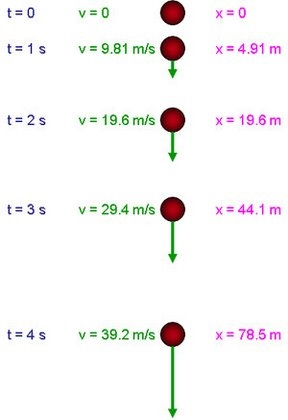
\includegraphics[scale=0.4]{images/freefall-timeline-large.jpg}
 % cinematica.png: 0x0 px, 300dpi, 0.00x0.00 cm, bb=
 \caption{Ilustración del tiempo de caída de un cuerpo.}\label{caidalibre2}
\end{figure}  
 
\subsection{Lanzamiento vertical:}

Este movimiento es de tipo MRUV que trata del lanzamiento de un cuerpo en línea recta hacia arriba en contra de la gravedad, y 
por tanto en este caso para cálculos la gravedad se toma como $g = -9.8 m/s^2$, se nota el signo negativo por cuanto en este caso 
el movimiento es retardado y la fuerza de la gravedad está encontra del movimiento. Obviamente para que ocurra este movimiento el 
cuerpo lanzado debe partir con una velocidad inicial diferente de cero ($v_0 = 0$), y así mismo la velocidad alcanzará su valor 
mínimo de cero donde se dice que el cuerpo ha alcanzado su altura máxima ($h_{max}$) y ya no sube más, y posteriormente bajará 
con 
un movimiento de caída libre que parte del reposo.
 
\begin{figure}[ht]
 \centering
 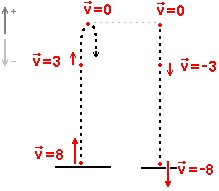
\includegraphics[scale=0.7]{images/lanzamientovertical.jpg}
 % cinematica.png: 0x0 px, 300dpi, 0.00x0.00 cm, bb=
 \caption{Ilustración del lanzamiento vertical.}\label{lanzamientov}
\end{figure}   
 
Es importante mencionar que cuando cuerpo realiza un lanzamiento vertical, este movimiento tiene cierta simetría con la caída 
libre que luego realizará una vez que alcanze la altura máxima, debido a que esta bajo la mismo módulo de la aceleración de la 
gravedad y que además recorre la misma distancia (altura), y por tanto el tiempo que demorá en subir el cuerpo (tiempo de subida: 
$t_s$) es el mismo tiempo que demora en bajar (tiempo de bajada: $t_b$).

\subsection{Problemas de caída libre y lanzamiento vertical}

\begin{enumerate}
 \item Supongamos que arrojamos una piedra hacia arriba, ¿a que velocidad la tenemos que lanzar para que alcance una altura máxima
de 32 metros?
\item Hallar la velocidad con que fue lanzado un cuerpo hacia arriba si ésta se reduce a la tercera parte cuando ha subido 29.4 m.
\item Un tipo está parado a 20 m de altura. Calcular qué tiempo tarda y con qué velocidad toca el suelo una piedra si el tipo:
\begin{itemize}
 \item[a.] La deja caer.
 \item[b.] La tira para abajo con V0 = 10 m/s.
\end{itemize}
\item Se lanza un cuerpo hacia arriba con una velocidad de 24,5 m/s desde un punto a 68,6 metros por encima del suelo. Halla:

\begin{itemize}
 \item[a.] La altura máxima que alcanza el cuerpo.
 \item[b.] El tiempo necesario para volver al punto de lanzamiento.
 \item[c.] La velocidad de llegada al suelo.
 \item[d.] El tiempo total en el aire.
\end{itemize}

\item Determina la velocidad con que fue lanzado un cuerpo hacia arriba si ésta se reduce a la tercera 
parte cuando ha subido 
29.4 m.

\item  Se deja caer una
 piedra desde lo alto de un edificio de 40 m de altura, ¿con que velocidad llegará al suelo?

\item  Una piedra es lanzada verticalmente
 hacia arriba con una velocidad de 98 m/s. ¿A qué altura llegará?

\item Un cuerpo se lanza verticalmente hacia arriba desde una ventana y luego de 4 segundos triplica su velocidad. Hallar la 
máxima altura alcanzada por el cuerpo respecto al lugar de lanzamiento.
\item Una esfera se deja caer desde 80 m de altura y al rebotar en el piso se eleva siempre la cuarta parte de la altura 
anterior. 
¿Qué tiempo ha transcurrido hasta que se produce el tercer impacto?.
\item Un cuerpo cae libremente desde el reposo. La mitad de su caída se realiza en el último segundo, calcular el tiempo total.

\item Un cuerpo se suelta desde una altura H. ¿Con qué velocidad llegará al suelo?.

\item Desde la boca de un pozo de 50 metros de profundidad, ¿a qué velocidad hay que lanzar una
 piedra para que llegue al fondo 
en 2 segundos?

\item Lanzamos hacia arriba un objeto desde la altura de 1,5 m y con una velocidad de 24,5 m/s.
 Determina la posici´on y la 
velocidad al instante de 3 segundos.


\item  Un cuerpo parte del reposo con una aceleración de $5 m/s^2$
.
 ¿Cuál es la distancia recorrida durante el octavo segundo 
del recorrido?

\item  Un niño deja caer una piedra desde lo alto de un árbol de 5
 m del suelo. Simultáneamente, otro niño lanza una piedra 
desde el suelo hacia arriba con una
 velocidad de 3 m/s. ¿A qué distancia del suelo coinciden las dos piedras en sus respectivas

trayectorias?

\item  Desde una altura de 200
 m se deja caer un cuerpo, y simultáneamente desde el suelo se lanza un cuerpo con una
 velocidad 
de 20 m/s hacia arriba. ¿Cuándo la distancia entre ellos es de 20m?.


\item Un niño deja caer una piedra desde lo alto de un árbol de 4 m del suelo. Simultáneamente,
 otro niño lanza una piedra desde 
el suelo hacia arriba con una velocidad de $6 m/s$
. ¿A qué distancia del
 suelo coinciden las dos piedras en sus respectivas 
trayectorias?

\item A una niña se le cae una pelota desde el quito piso de un edificio, a 15 metros del suelo.
 El vecino del tercero, a 9 m 
del suelo la ve pasar. Calcular: a) El tiempo que tarda en llegar al suelo, b) su
 velocidad al pasar por el tercer piso.


\item Nahiara deja caer una moneda a un pozo y escucha el sonido del agua 2,5 s después de
 iniciarse la caída. Halla: a) La 
profundidad del pozo y, b) la velocidad con la que llega al agua (La velocidad del sonido $340 m/s$).

\end{enumerate}
